\subsection{Modélisation}

	\subsubsection{Exemple de requête sous Neo4j}
	Neo4j est une \bddGraphe{} qui est actuellement la plus populaire de sa catégorie. Pour comprendre comment écrire les requêtes sous Neo4j, il faut tout d'abord être familier avec le concept de graphe. Pour simplifier, un graphe connecte des nœuds (des \enquote{entités}) entre eux à l'aide de liens, qui symbolisent les relations. On peut stocker les informations que l'on souhaite dans les nœuds ou dans les liens.\\

	Voici un exemple de graphe qui représente une partie des relations du film \enquote{\textit{The Matrix}} et \enquote{\textit{Cloud Atlas}} sur la figure \ref{grapheNeo4j}. On y retrouve les différents acteurs et le réalisateur du film. Les nœuds sont les personnes et les liens sont les relations qu'ils ont par rapport au film. Dans notre cas, il y a en a que deux :
	\vspace{5px}
	\begin{itemize}
		\item \textit{DIRECTED} : la personne est un des réalisateurs du film pointé par la liaison ; 
		\item \textit{ACTED\_IN} : la personne est un acteur du film pointé par la liaison. 
	\end{itemize}

	\begin{figure}[H]
		\centering
		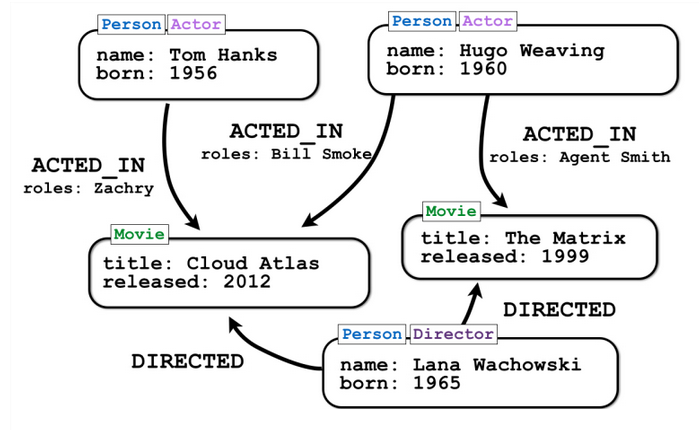
\includegraphics[width=0.9\textwidth]{images/graphe.png}
		\caption{Un graphe représentant une partie des relations pour les films \enquote{\textit{The Matrix}} et \enquote{\textit{Cloud Atlas}}.\cite{grapheNeo4j}}
		\label{grapheNeo4j}
	\end{figure}

	Si l'on veut, à partir de ce graphe, trouver tous les acteurs jouant dans le film \enquote{\textit{The Matrix}} et le rôle qu'ils jouent, la requête à écrire est présentée dans la figure~\ref{requeteNeo4j}.

	\begin{figure}[H]
		\centering
		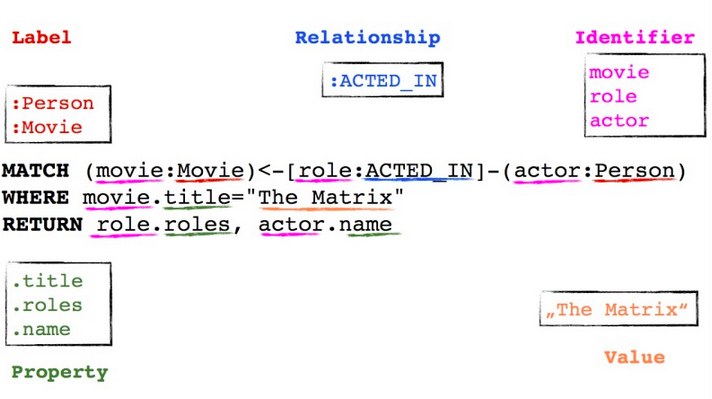
\includegraphics[width=0.9\textwidth]{images/requeteNeo4j.png}
		\caption{Trouver tous les acteurs du film \enquote{\textit{The Matrix}}.\cite{grapheNeo4j}}
		\label{requeteNeo4j}
	\end{figure}

\subsection{Cas d'utilisation}
	Une \bddGraphe{} n'a pas pour vocation à être utilisée comme seul moteur de stockage, sauf dans le cas d'applications très spécifiques ou de modules d'un système d'information. Les bases de données orientée graphe sont adaptées lorsque les données manipulées possèdent un grand nombre de liaisons entre elles. Pour rappel, les bases de données orientée graphe accordent une importance égale pour les nœuds et les relations entre ces nœuds. Voici quelques cas d'utilisation où une \bddGraphe{} est particulièrement adaptée\footnote{Ces exemples sont tirés du site officiel de Neo4j : \url{http://neo4j.com}} :

	\begin{itemize}
	 	\item \textbf{Modélisation de réseaux.} Les interconnexions entre des équipements, virtuels ou physiques, peuvent être représenter parfaitement par un graphe. On peut imaginer représenter un réseau de distribution d'eau ou un réseau mobile par exemple. Une fois le système modélisé on peut effectuer des analyses d'impact de panne, détecter la source d'un incident, améliorer la qualité de service, prévoir des maintenances\dots
	 	\item \textbf{Réseaux sociaux.} La famille, les amis, les followers sont parfaitement représentés dans un graphe social qui permet de mettre en évidence les comportements, les influences et les groupes implicites. On peut alors réaliser des recommandations d'amis, des suggestions de partage et de l'analyse d'influence.
	 	\item \textbf{Gestion d'accès.} Qui vous êtes, à qui vous appartenez et ce que vous êtes autorisé à faire dépend des relations entre vous, une entreprise et un système.
	 	\item \textbf{Organisation hiérarchique.} Qui dirige qui ? Qui est responsable de qui ? Qui finance qui ? Toutes ces questions reviennent souvent pour une entreprise ayant une taille conséquence. Ces relations peuvent être modélisées dans une \bddGraphe{}.
	 \end{itemize} 

\subsection{Acteurs principaux}
	La popularité des bases de données est donnée par DB-engines\cite{db_engines_key_value} pour le mois de novembre 2014.

	\begin{enumerate}
		\item \textbf{Neo4j}. Première version en 2007, écrit en Java, open-source sous licence GPLv3. Certains modules (comme la haute disponibilité) sont payants et sous licence AGPLv3. Le développement est assuré par Neo Technology. Utilisé par SFR, Ebay, HP, National Geographic, Walmart\dots
		\item \textbf{Titan.} Première version en 2012, écrit en Java, open-source sous licence Apache 2. Le développement est assuré par Aurelius, une équipe d'ingénieurs qui aide au déploiement de Titan. Peut respecter les propriétés ACID\ref{subsec:proprietesACID}.
		\item \textbf{OrientDB.} Première version en 2010, écrit en Java, open-source sous licence Apache 2. C'est une base de données orientée documents mais les relations sont stockées dans un graphe. Le système peut être interrogé en SQL.
	\end{enumerate}
